\documentclass[16pt]{article}

\usepackage{amsmath,amssymb,amsthm,amsfonts,amscd}
\usepackage{showlabels}
\usepackage{color}
\usepackage{hyperref}
\usepackage[numeric]{amsrefs}
\usepackage{graphicx}

\usepackage{pgf,tikz}
\usetikzlibrary{angles,quotes}


\usepackage[framemethod=TikZ]{mdframed}
%\usepackage[framemethod=default]{mdframed}

%\mdfdefinestyle{box}{%
%rightline=true,
%innerleftmargin=10,
%innerrightmargin=10,
%frametitlerule=true,
%frametitlerulecolor=blue,
%frametitlebackgroundcolor=white,
%frametitlerulewidth=2pt}

\mdfdefinestyle{TheoremFrame}{%
    linecolor=blue,
    outerlinewidth=1,
    roundcorner=15,
    innertopmargin= \baselineskip,
    innerbottommargin= \baselineskip,
    innerrightmargin=10,
    innerleftmargin=10,
    backgroundcolor=white}
    
\mdfdefinestyle{ProofFrame}{%
    linecolor=red,
    outerlinewidth=1,
    roundcorner=15,
    innertopmargin= \baselineskip,
    innerbottommargin= \baselineskip,
    innerrightmargin=10,
    innerleftmargin=10,
    backgroundcolor=white}
    
    
\setlength{\oddsidemargin}{0cm}
\setlength{\evensidemargin}{0cm}
\setlength{\marginparwidth}{0in}
\setlength{\marginparsep}{0in}
\setlength{\marginparpush}{0in}
\setlength{\topmargin}{0in}
\setlength{\headheight}{0pt}
\setlength{\headsep}{0pt}
\setlength{\footskip}{.3in}
\setlength{\textheight}{9.2in}
\setlength{\textwidth}{6.0in}
\setlength{\parskip}{0.25pt}
\setlength{\parindent}{0.25in}

    
\newlength\tindent
\setlength{\tindent}{\parindent}
\setlength{\parindent}{0pt}
\renewcommand{\indent}{\hspace*{\tindent}}

\newtheorem*{nthm}{Theorem}
\newtheorem*{nlem}{Lemma}
\newtheorem*{nprop}{Proposition}
\newtheorem*{ncor}{Corollary}
\newtheorem*{nconj}{Conjecture}
\newtheorem*{nclaim}{Claim}
\theoremstyle{remark}
\newtheorem*{define}{Definition}
\newtheorem*{nrem}{Remarks}
\newtheorem*{notation}{Notation}
\newtheorem*{note}{Note}
\newtheorem*{ex}{Example}
\newtheorem*{imt}{Important}
\newtheorem*{fact}{Fact}
\newcommand{\vs}{\vspace{0.1in}}
\newcommand{\Lim}[1]{\raisebox{0.5ex}{\scalebox{0.8}{$\displaystyle \lim_{#1}\;$}}}
\allowdisplaybreaks

\title{\vspace*{-1.5cm}Trig Substitution}

\author{Stephen Styles}


\begin{document}

\maketitle

For integrals of the form $\displaystyle{\int (a^2 -b^2x^2)^n \,dx}$ use $\displaystyle{x=\frac{a\sin(\theta)}{b}}$ as your substitution. From there we get the triangle:
\begin{center}
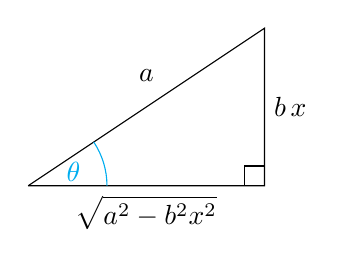
\begin{tikzpicture}[
  my angle/.style={
    every pic quotes/.append style={text=cyan},
    draw=cyan,
    angle radius=1cm,
  }]
  \coordinate (C) at (-1.5,-1);
  \coordinate  (A) at (1.5,-1);
  \coordinate  (B) at (1.5,1);
  \draw (C) -- node[shift={(0,0.4)}] {$a$} (B) -- node[right] {$b\,x$} (A) -- node[below] {$\displaystyle{\sqrt{a^2-b^2x^2}}$} (C);
  \draw (A) +(-.25,0) |- +(0,.25);
  \pic [my angle, "$\theta$"] {angle=A--C--B};
\end{tikzpicture}
\end{center}

A useful trig identity for these questions is $r^2\sin^2(x)+ r^2 \cos^2(x) = r^2$.

\begin{mdframed}[style=TheoremFrame]
Example 1: Find $\displaystyle{\int \frac{x-2}{\sqrt{9+4x-x^2}}\, dx  }$\\

\textit{Solution:}
\begin{align*}
\int \frac{x-2}{\sqrt{5+4x-x^2}}\, dx  &= \int \frac{x-2}{\sqrt{9-4+4x-x^2}}\, dx\\[1.5ex]
&= \int \frac{x-2}{\sqrt{9-(x-2)^2}}\, dx
\end{align*}
\begin{center}
Let $\displaystyle{x-2 = 3\sin(\theta)}$, then $dx = 3 \cos(\theta)\, d\theta$.
\end{center}
\begin{align*}
\int \frac{x-2}{\sqrt{5+4x-x^2}}\, dx  &= \frac{1}{3} \int \frac{3\sin(\theta)\cos(\theta)}{\sqrt{9 - (3\sin(\theta))^2}}\, d\theta\\[1.5ex]
&= \int \frac{\sin(\theta)\cos(\theta)}{\sqrt{9 - 9\sin^2(\theta)}}\, d\theta\\[1.5ex]
&= \int \frac{\sin(\theta)\cos(\theta)}{\sqrt{9\cos^2(\theta)}}\, d\theta\\[1.5ex]
&= \frac{1}{3}\int \frac{\sin(\theta)\cos(\theta)}{\cos(\theta)}\, d\theta\\[1.5ex]
&= \frac{1}{3} \int \sin(\theta) \, d\theta\\[1.5ex]
&= -\frac{1}{3} \cos(\theta) + C\\[1.5ex]
&= \frac{-\sqrt{9-(x-2)^2}}{27} + C
\end{align*}
\end{mdframed}
\newpage
\begin{enumerate}

\item $\displaystyle{\int \sqrt{4-25x^2}\, dx}$
\begin{mdframed}[style=TheoremFrame]
\textit{Solution:}

\begin{center}
Let $\displaystyle{x = \frac{2}{5}\sin(\theta) }$, then $\displaystyle{ dx = \frac{2}{5}\cos(\theta) \, d\theta }$.
\end{center}
\begin{align*}
\int \sqrt{4-25x^2}\, dx &= \frac{2}{5}\int \sqrt{4 - 25\bigg(\frac{2}{5} \sin(\theta)\bigg)^2} \cos(\theta) \, d\theta\\[2ex]
&= \frac{2}{5}\int \sqrt{4 - 25\bigg(\frac{2}{5} \sin(\theta)\bigg)^2} \cos(\theta) \, d\theta\\[2ex]
&= \frac{2}{5}\int \sqrt{4 - 4 \sin^2(\theta)} \cos(\theta) \, d\theta\\[2ex]
&= \frac{2}{5}\int \sqrt{4 \cos^2(\theta)} \cos(\theta) \, d\theta\\[2ex]
&= \frac{4}{5}\int \cos^2(\theta) \, d\theta\\[2ex]
&= \frac{4}{5}\int \frac{1+\cos(2\theta)}{2} \, d\theta\\[2ex]
&= \frac{2}{5}\int 1+\cos(2\theta) \, d\theta\\[2ex]
&= \frac{2}{5}\bigg( \theta +\frac{\sin(2\theta)}{2} \bigg) +C\\[2ex]
&= \frac{2}{5}\bigg( \theta +\frac{2\sin(\theta)\cos(\theta)}{2} \bigg) +C\\[2ex]
&= \frac{2}{5}\bigg( \theta +\sin(\theta)\cos(\theta) \bigg) +C\\[2ex]
&= \frac{2}{5}\bigg( \sin^{-1}\bigg(\frac{5x}{2}\bigg) +\frac{\sqrt{4-25x^2}}{2}\frac{5x}{2}\bigg)+C\\[2ex]
&= \frac{2}{5} \sin^{-1}\bigg(\frac{5x}{2}\bigg) +\frac{x\sqrt{4-25x^2}}{2}+C
\end{align*}
\end{mdframed}
\newpage
\item $\displaystyle{\int \frac{1}{\sqrt{1-9x^2}} \, dx}$
\begin{mdframed}[style=TheoremFrame]
\textit{Solution:}

\end{mdframed}
\newpage
\item $\displaystyle{\int \frac{1}{x^4\sqrt{9-x^2}}\, dx}$
\begin{mdframed}[style=TheoremFrame]
\textit{Solution:}

\end{mdframed}
\newpage
\item $\displaystyle{\int \frac{\sqrt{16-x^2}}{x^2} \,dx}$
\begin{mdframed}[style=TheoremFrame]
\textit{Solution:}

\end{mdframed}
\newpage

\end{enumerate}

For integrals of the form $\displaystyle{\int (a^2 +b^2x^2)^n \,dx}$ use $\displaystyle{x=\frac{a\tan(\theta)}{b}}$ as your substitution. The triangle we get from this substitution is:

\begin{center}
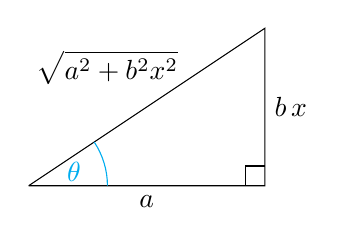
\begin{tikzpicture}[
  my angle/.style={
    every pic quotes/.append style={text=cyan},
    draw=cyan,
    angle radius=1cm,
  }]
  \coordinate (C) at (-1.5,-1);
  \coordinate  (A) at (1.5,-1);
  \coordinate  (B) at (1.5,1);
  \draw (C) -- node[shift={(-0.5,0.5)}] {$\displaystyle{\sqrt{a^2+b^2x^2}}$} (B) -- node[right] {$b\,x$} (A) -- node[below] {$a$} (C);
  \draw (A) +(-.25,0) |- +(0,.25);
  \pic [my angle, "$\theta$"] {angle=A--C--B};
\end{tikzpicture}
\end{center}

A useful identity for these questions is $r^2 + r^2 \tan^2(x) = r^2 \sec^2(x)$.

\begin{mdframed}[style=TheoremFrame]
Example 2: Find $\displaystyle{ \int \frac{e^{2x}}{\sqrt{e^{4x}+1}} \, dx }$\\

\textit{Solution:}
\begin{center}
Let $e^{2x} = \tan(\theta)$, then $2\, e^{2x}\, dx = \sec^2(\theta)\, d\theta $.
\end{center}
\begin{align*}
\int \frac{e^{2x}}{\sqrt{e^{4x}+1}} \, dx &= \frac{1}{2} \int \frac{\sec^2(\theta)}{\sqrt{\tan^2(\theta)+1}} \, d\theta \\[2ex]
&= \frac{1}{2} \int \frac{\sec^2(\theta)}{\sqrt{\sec^2(\theta)}} \, d\theta \\[2ex]
&= \frac{1}{2} \int \sec(\theta)\, d\theta \\[2ex]
&= \frac{1}{2} \ln\big| \sec(\theta) + \tan(\theta) \big| + C\\[2ex]
&= \frac{1}{2} \ln\bigg| \sqrt{e^{4x}+1} + e^{2x} \bigg| + C
\end{align*}

Note: This integral can also be solved using inverse hyperbolic trig functions.

\begin{center}
Let $u = e^{2x}$, then $du = 2 \, e^{2x} \, dx$.
\end{center}
\begin{align*}
\int \frac{e^{2x}}{\sqrt{e^{4x}+1}} \, dx &= \frac{1}{2} \int \frac{1}{\sqrt{u^2+1}} \, du \\[2ex]
&= \frac{1}{2} \sinh^{-1} (u) + C\\[2ex]
&= \frac{1}{2} \sinh^{-1} \big(e^{2x}\big) + C
\end{align*}
\end{mdframed}
\newpage
\begin{enumerate}
\item $\displaystyle{\int \frac{\sqrt{9+x^2}}{x^4}\, dx}$
\begin{mdframed}[style=TheoremFrame]
\textit{Solution:}

\end{mdframed}

\item $\displaystyle{\int \frac{3x}{x^2+10x+29}\, dx}$
\begin{mdframed}[style=TheoremFrame]
\textit{Solution:}

\end{mdframed}
\newpage
\item $\displaystyle{\int_{-1}^{1} \frac{1}{(1+x^2)^2}\, dx}$
\begin{mdframed}[style=TheoremFrame]
\textit{Solution:}

\end{mdframed}

\item $\displaystyle{\int \frac{1}{\sqrt{25x^2+16}}\, dx}$
\begin{mdframed}[style=TheoremFrame]
\textit{Solution:}

\end{mdframed}
\newpage
\end{enumerate}
For integrals of the form $\displaystyle{\int (b^2x^2 -a^2)^n \,dx}$ use $\displaystyle{x=\frac{a\sec(\theta)}{b}}$ as your substitution. The triangle we get from this substitution is:

\begin{center}
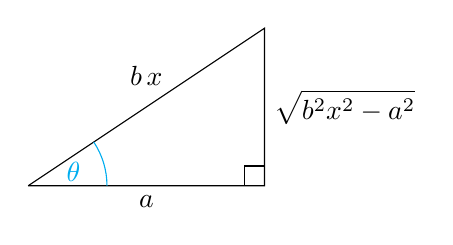
\begin{tikzpicture}[
  my angle/.style={
    every pic quotes/.append style={text=cyan},
    draw=cyan,
    angle radius=1cm,
  }]
  \coordinate (C) at (-1.5,-1);
  \coordinate  (A) at (1.5,-1);
  \coordinate  (B) at (1.5,1);
  \draw (C) -- node[shift={(0,0.4)}] {$b\,x$} (B) -- node[right] {$\displaystyle{\sqrt{b^2x^2-a^2}}$} (A) -- node[below] {$a$} (C);
  \draw (A) +(-.25,0) |- +(0,.25);
  \pic [my angle, "$\theta$"] {angle=A--C--B};
\end{tikzpicture}
\end{center}
A useful identity for these questions is $r^2 \sec^2 (x) - r^2 = r^2 \tan^2(x)$

\begin{mdframed}[style=TheoremFrame]
Example 3: Find $\displaystyle{ \int x^2 \sqrt{x^2 - 10x} \, dx }$\\

\textit{Solution:}

\begin{align*}
\int (x-5) \sqrt{x^2 - 10x} \, dx &= \int x^2 \sqrt{x^2 - 10x+ 25 - 25} \, dx \\[1.5ex]
&= \int x^2 \sqrt{(x-5)^2 - 25} \, dx\\
\end{align*}
\begin{center}
Let $x -5 = 5\sec(\theta)$, then $dx = 5 \sec(\theta) \tan(\theta) \, d\theta$.
\end{center}
\begin{align*}
\int (x-5) \sqrt{x^2 - 10x} \, dx &= 25 \int \sec(\theta) \sqrt{(5\sec(\theta))^2 - 25} \sec(\theta) \tan(\theta) \, d\theta\\[1.5ex]
&= 25 \int \sec^2(\theta) \sqrt{25\sec(\theta)^2 - 25}\tan(\theta) \, d\theta\\[1.5ex]
&= 25 \int \sec^2(\theta) \sqrt{25\tan(\theta)^2}\tan(\theta) \, d\theta\\[1.5ex]
&= 125 \int \sec^2(\theta)\tan^2(\theta) \, d\theta
\end{align*}
\begin{center}
Let $u = \tan(\theta)$, then $du = \sec^2(\theta) \, d\theta$.
\end{center}
\begin{align*}
\int (x-5) \sqrt{x^2 - 10x} \, dx &= 125 \int u^2 \, du\\[1.5ex]
&= \frac{125u^3}{3}+C\\[1.5ex]
&= \frac{125\tan^3(\theta)}{3}+C\\[1.5ex]
&= \frac{125}{3} \bigg(\frac{x^2-10x}{5} \bigg)^3 + C\\[1.5ex]
&= \frac{(x^2+10x)^{3/2}}{3} + C
\end{align*}
\end{mdframed}

\begin{enumerate}
\item $\displaystyle{\int \frac{1}{\sqrt{25x^2-1}}\, dx}$
\begin{mdframed}[style=TheoremFrame]
\textit{Solution:}

\end{mdframed}
\item $\displaystyle{\int \frac{\sqrt{16x^2-9}}{x}\, dx}$
\begin{mdframed}[style=TheoremFrame]
\textit{Solution:}

\end{mdframed}
\newpage
\item $\displaystyle{\int \frac{1}{x^2\sqrt{x^2-36}}\, dx}$
\begin{mdframed}[style=TheoremFrame]
\textit{Solution:}

\end{mdframed}

\item $\displaystyle{\int \frac{x}{\sqrt{x^2-4}}\, dx}$
\begin{mdframed}[style=TheoremFrame]
\textit{Solution:}

\end{mdframed}


\end{enumerate}


\end{document}